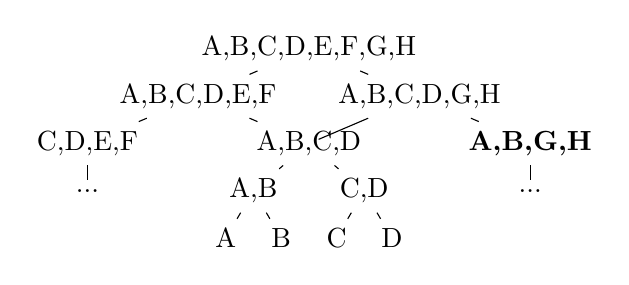
\begin{tikzpicture}
[level 1/.style={sibling distance=8em},
level 3/.style={sibling distance=4em},
level 4/.style={sibling distance=2em}, level distance=0.6cm
]
    \tikzstyle{n}=[draw, fill, circle]

    \node (a) at (0,0) {A,B,C,D,E,F,G,H}
        child { node {A,B,C,D,E,F}
            child { node {C,D,E,F}
                % child {node { }}
                child {node {...}}
                % child {node { }}
                % child {node { }}
                }
            child { node[sibling distance=2em] {A,B,C,D}
                child {node {A,B}
                    child {node {A}}
                    child {node {B}}
                    }
                child {node {C,D}
                    child {node {C}}
                    child {node {D}}
                    }
                }
            }
        child { node {A,B,C,D,G,H}
            child { node { } }
            child { node {{\bf A,B,G,H}}
                % child {node { }}
                child {node {...}}
                % child {node { }}
                % child {node { }}
            }
        };
\end{tikzpicture}
